\documentclass[11pt]{article}
\usepackage[utf8]{inputenc}
\usepackage{geometry}
\usepackage{booktabs}
\usepackage{graphicx}
\usepackage{hyperref}
\usepackage{amsmath}
\usepackage{amssymb}
\usepackage{caption}

\title{Preferences in AI Project Report}
\author{Pratik Deshmukh}
\date{\today}

\begin{document}

\maketitle

\section{Introduction}
This report presents experiments on free-riding in sequential decision-making
under different \emph{statistical cultures}, following the framework of
\cite{lackner2023freeriding}.

\section{Background}

\subsection{Multi-Issue Model}
We study sequential decision-making in \emph{multi-issue elections}, where a set
of voters must make a series of binary (yes/no) or multi-candidate decisions,
one per issue. Each voter submits approval preferences for all candidates on
each issue. A voting rule is then applied issue by issue to determine the
collective outcome.

\subsection{Voting Rules}
We focus on two families of rules:
\begin{itemize}
    \item \textbf{Sequential Utilitarian Rule:} selects in each issue the
    candidate with the highest total number of approvals.
    \item \textbf{Thiele-Based Rules:} a general class where voter satisfaction
    decreases marginally as more of their approved candidates are selected.  
    Examples include:
    \begin{itemize}
        \item \emph{Proportional Approval Voting (PAV)} with harmonic weights
        $(1, \tfrac{1}{2}, \tfrac{1}{3}, \dots)$,
        \item \emph{Chamberlin--Courant (CC)} with weights $(1,0,0,\dots)$.
    \end{itemize}
    \item \textbf{OWA-Based Rules:} aggregate voter satisfaction using Ordered
    Weighted Averages (OWAs). For instance:
    \begin{itemize}
        \item \emph{Leximin OWA:} maximizes the welfare of the worst-off voter,
        \item \emph{Mean OWA:} averages utilities across voters.
    \end{itemize}
\end{itemize}

\subsection{Statistical Cultures}
The way preferences are generated strongly influences experimental outcomes.
We consider four cultures:
\begin{itemize}
    \item \textbf{p-IC}: per-issue impartial culture, sampling preferences
    independently with probability $p$.
    \item \textbf{Disjoint Groups}: voters are divided into $g$ groups with
    internally aligned preferences.
    \item \textbf{Resampling Model}: preferences are generated by resampling
    with parameters $(p, \phi)$ controlling randomness and correlation.
    \item \textbf{Hamming Noise}: preferences are first generated from another
    culture and then perturbed by flipping approvals with small probability.
\end{itemize}

\subsection{Welfare and Risk Metrics}
We evaluate outcomes using two families of metrics:
\begin{itemize}
    \item \textbf{Welfare Metrics:}  
    \begin{itemize}
        \item \emph{Utilitarian welfare:} sum of utilities across all voters.  
        \item \emph{Egalitarian welfare:} minimum utility among all voters.  
        \item \emph{Nash welfare:} product of voter utilities (geometric balance).  
    \end{itemize}
    \item \textbf{Risk Metrics:}  
    \begin{itemize}
        \item \emph{Successes:} number of manipulations that improved the manipulator’s outcome.  
        \item \emph{Harms:} number of manipulations that backfired on the manipulator.  
        \item \emph{Success rate:} proportion of trials with a successful manipulation.  
        \item \emph{Harm rate:} proportion of trials with a harmful manipulation.  
    \end{itemize}
\end{itemize}

\section{Methodology}
We repeat the experiments from the paper but use several different statistical
cultures: impartial culture (p-IC), disjoint groups, the $(p, \phi)$-resampling
model, and the Hamming-noise model. For each, we run multiple seeds and compare
welfare and risk metrics under sequential utilitarian, seq-PAV, and seq-CC rules.

\subsection{Parameters}
For transparency, we explicitly document the parameters used in our experiments:

\begin{itemize}
    \item \textbf{p-IC}: resampling probabilities 
    $p \in \{0.25, 0.5, 0.75\}$, with each issue sampled independently.
    \item \textbf{Disjoint}: voters are partitioned into $g = 4$ fixed groups, 
    each with aligned preferences across all $k$ issues.
    \item \textbf{Resampling}: combinations of $(p,\phi)$ include 
    $(0.25, 0.25)$ and $(0.5, 0.75)$, where $p$ is the resampling probability 
    and $\phi$ controls correlation strength.
    \item \textbf{Hamming noise}: perturbations are introduced by flipping a 
    voter’s approval with probability $0.1$ or $0.2$ per issue, to model 
    random noise in preferences.
\end{itemize}
For all cultures, we fix the number of voters $n=50$, issues $k=10$, and
committee size $m=5$. Each configuration is run with 10 different random seeds.

\section{Results}
The combined results table is automatically generated by the experiment
pipeline. The table below is included directly from the output file:

\begin{table}[h!]
\centering
\resizebox{\textwidth}{!}{%
\input{tables/combined.tex}
}
\caption{Combined results across cultures and rules. Welfare metrics are
(utilitarian, egalitarian, Nash), while risk metrics include success and harm
rates.}
\label{tab:combined}
\end{table}

\subsection{Global Comparisons}

\begin{figure}[h!]
\centering
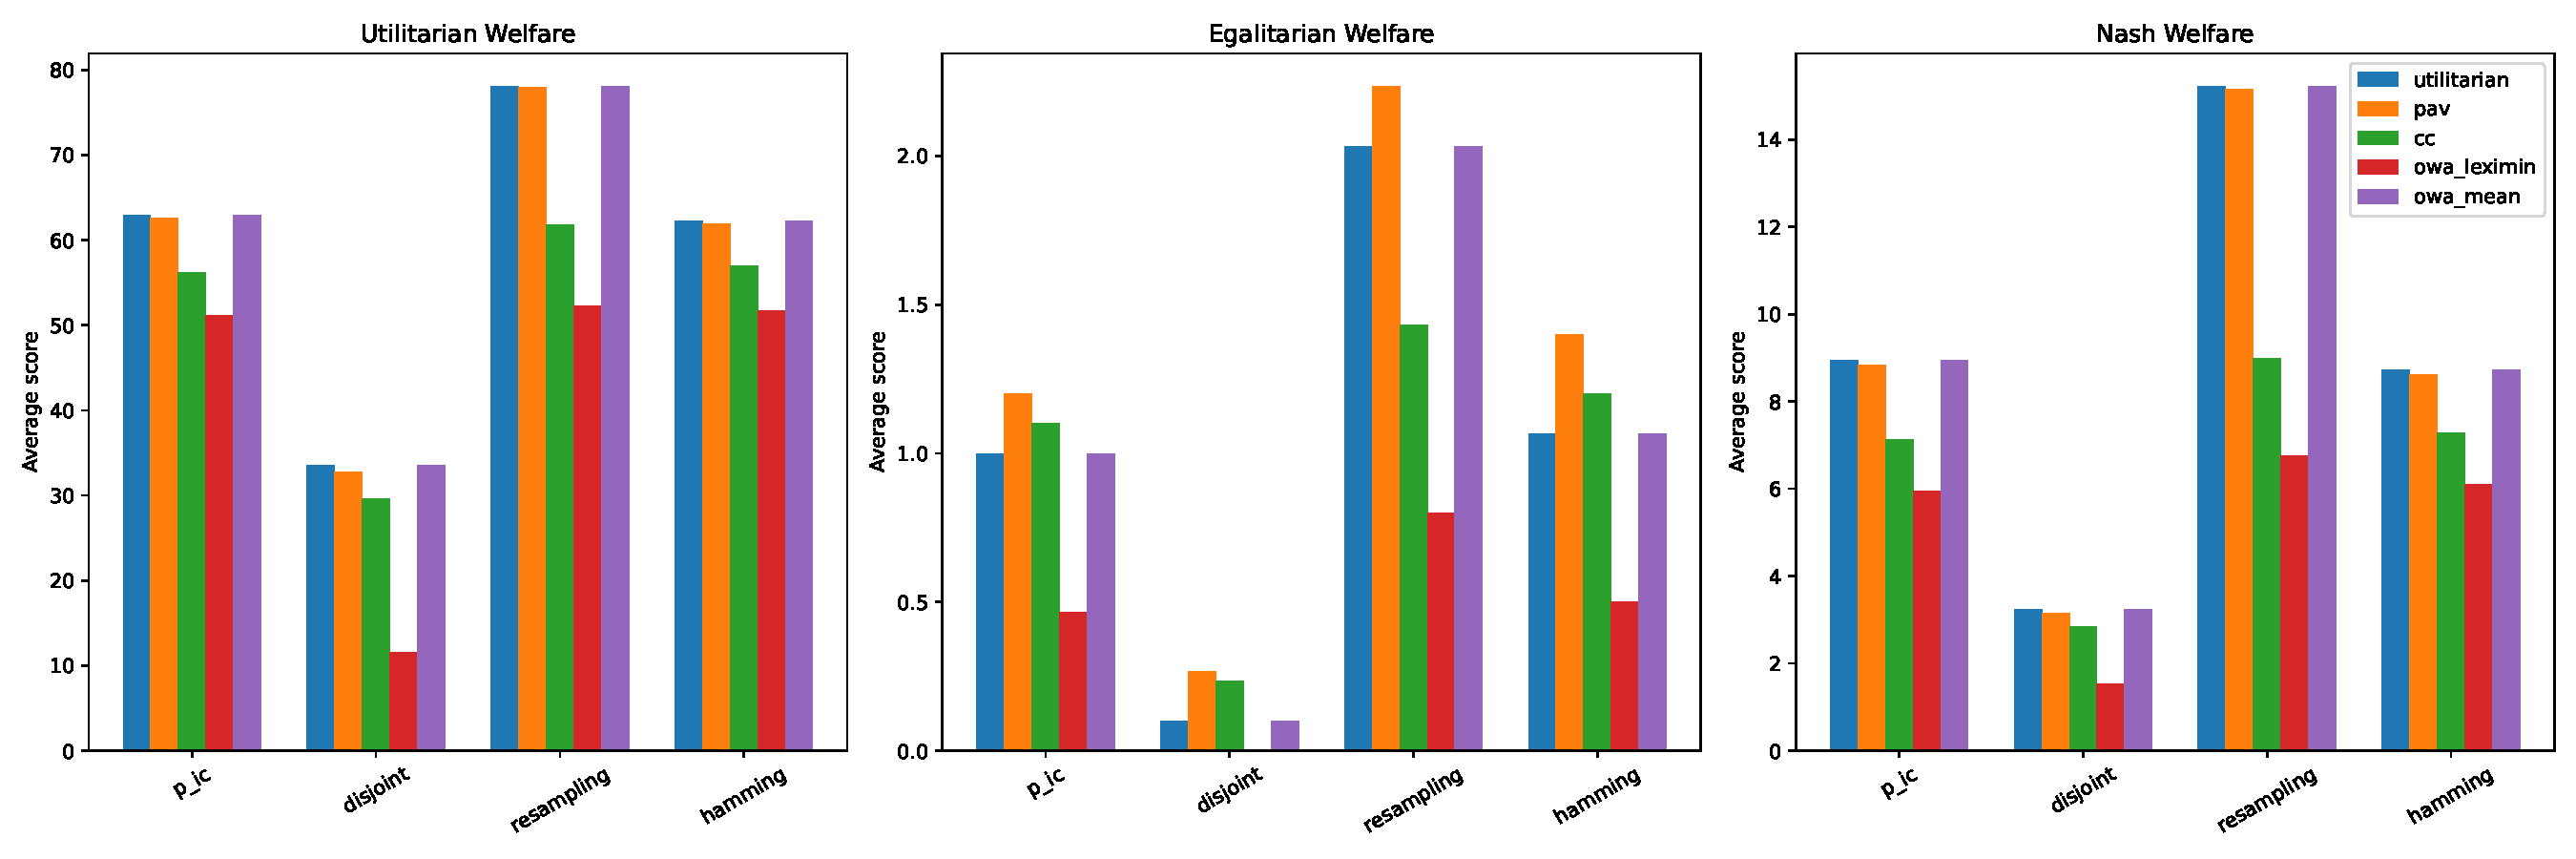
\includegraphics[width=\textwidth]{../figures/welfare_comparison_all.pdf}
\caption{Welfare metrics across cultures and rules. Each subplot shows utilitarian, egalitarian, or Nash welfare.}
\label{fig:welfare-global}
\end{figure}

\begin{figure}[h!]
\centering
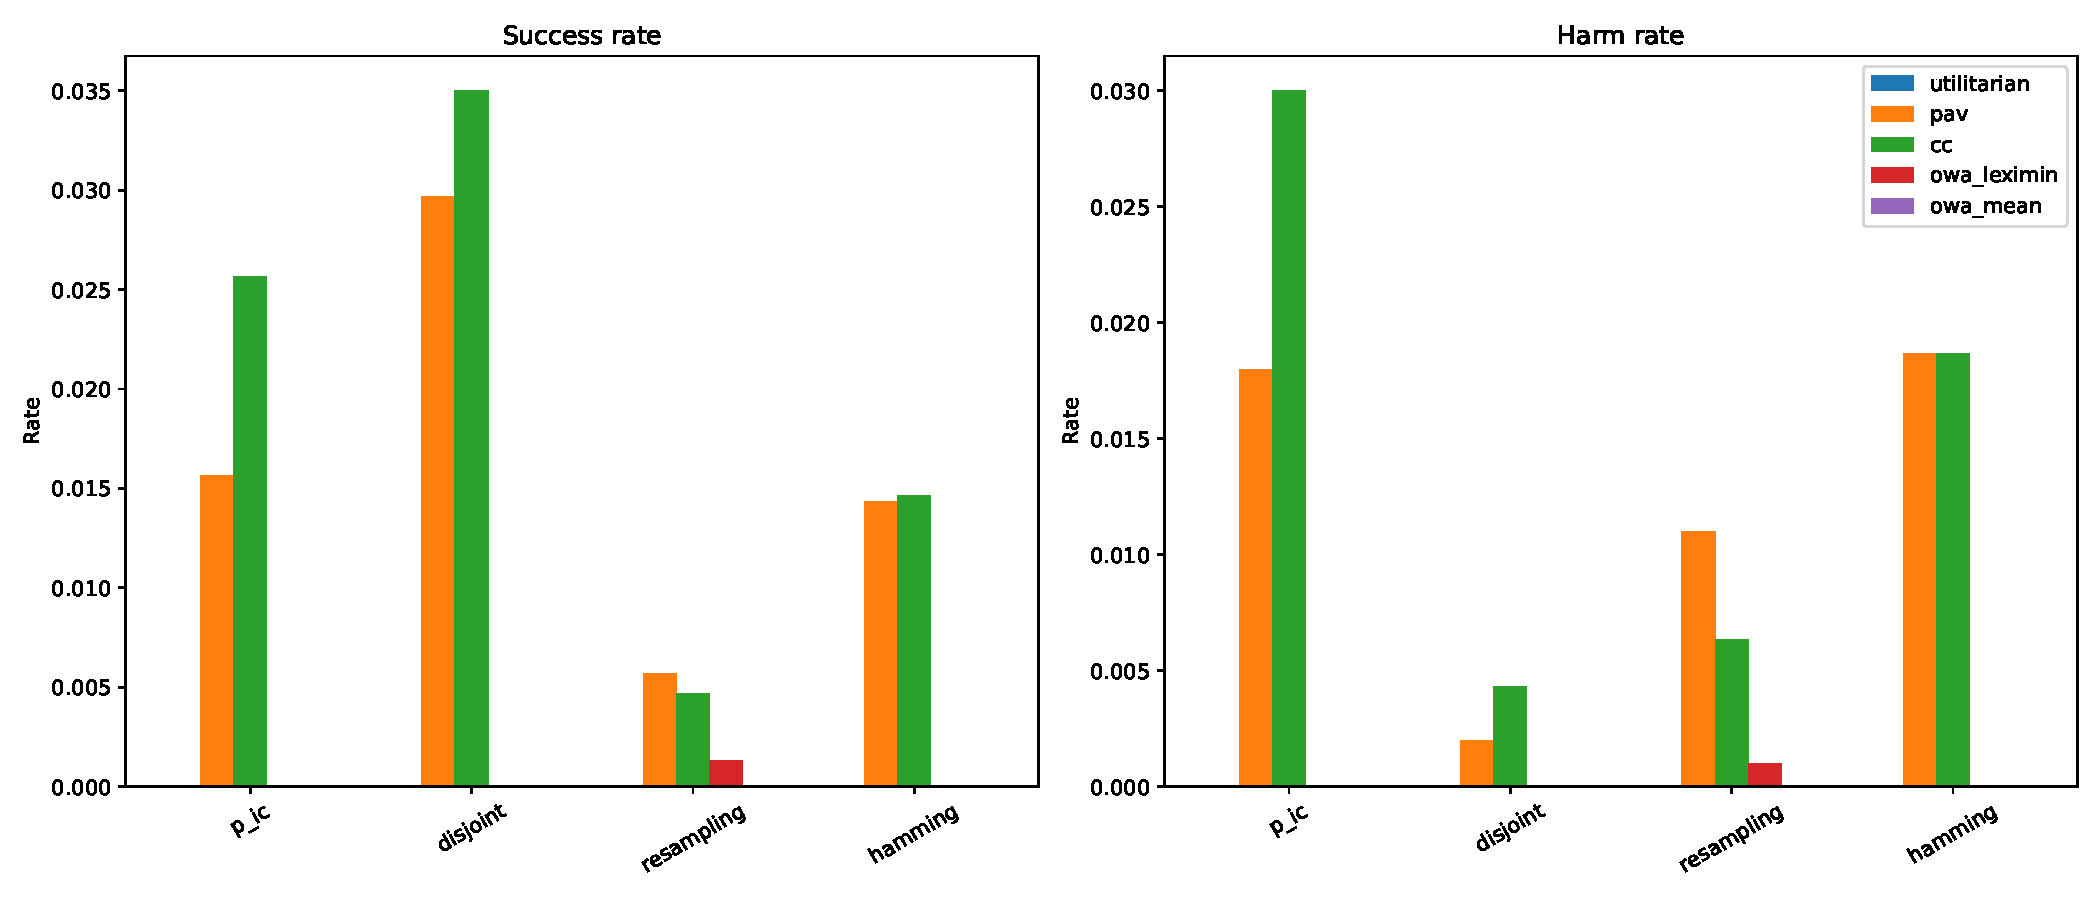
\includegraphics[width=\textwidth]{../figures/risk_comparison_all.pdf}
\caption{Manipulation risk (success and harm rates) across cultures and rules.}
\label{fig:risk-global}
\end{figure}

\section{Discussion}
Our experiments highlight the strong dependence of results on both the choice of
voting rule and the statistical culture used to generate preferences.

\paragraph{Effect of Statistical Cultures.}
The \emph{p-IC} culture yields relatively balanced welfare outcomes, but
manipulation risks are non-negligible (see Fig.~\ref{fig:welfare-global} and
Fig.~\ref{fig:risk-global}). The \emph{disjoint} model shows much lower welfare,
with preferences polarized across groups. The \emph{resampling} model produces
higher welfare but introduces manipulation opportunities. Finally, \emph{Hamming
noise} highlights robustness: small random flips can reduce manipulation
opportunities but also slightly lower welfare.

\paragraph{Effect of Voting Rules.}
The \emph{utilitarian rule} maximizes approvals but is highly exposed to
manipulation. Thiele rules provide different trade-offs: \emph{PAV} offers
proportionality with some manipulation risk, while \emph{CC} heavily rewards
first approvals and thus reduces manipulation success at the cost of lower
welfare. OWA rules show further trade-offs: \emph{Leximin} minimizes risk for
the worst-off voter, while the \emph{mean OWA} balances welfare and risk.

\paragraph{Risk Metrics.}
Disjoint cultures create fewer opportunities for free-riding, while resampling
and p-IC allow more. Harm rates are never negligible, confirming that voters
attempting to free-ride risk worsening their outcomes.

\section{Conclusion}
Our experiments confirm that the choice of statistical culture strongly
influences both welfare outcomes and robustness of voting rules to manipulation.
Cultures such as disjoint groups lead to low welfare but reduced manipulation
success, while resampling and p-IC generate higher welfare but greater
susceptibility to free-riding. The introduction of Hamming noise shows that
even small perturbations can alter both welfare and risk profiles, highlighting
the fragility of certain rules.

Across voting rules, utilitarian aggregation achieves high welfare but exposes
itself to manipulation. Thiele-based rules (PAV, CC) and OWA-based rules
(leximin, mean) illustrate trade-offs: reducing manipulation success comes at
the expense of utilitarian efficiency.

Future work should extend these experiments by exploring richer grids of
parameters $(p,\phi)$, noise rates, and group structures, as well as alternative
OWA weightings. Replicating the visualization style of
\cite{lackner2023freeriding} with plots would also allow direct side-by-side
comparison of manipulation risk across rules.

\section*{Repository}
The full project code and report sources are available at: \\
\href{https://github.com/inquisitour/preferences-in-ai}{github.com/inquisitour/preferences-in-ai}

\clearpage
\listoffigures

\appendix
\section{Per-Culture Figures}

\subsection{Per-Issue Impartial Culture (p-IC)}

\begin{figure}[h!]
\centering
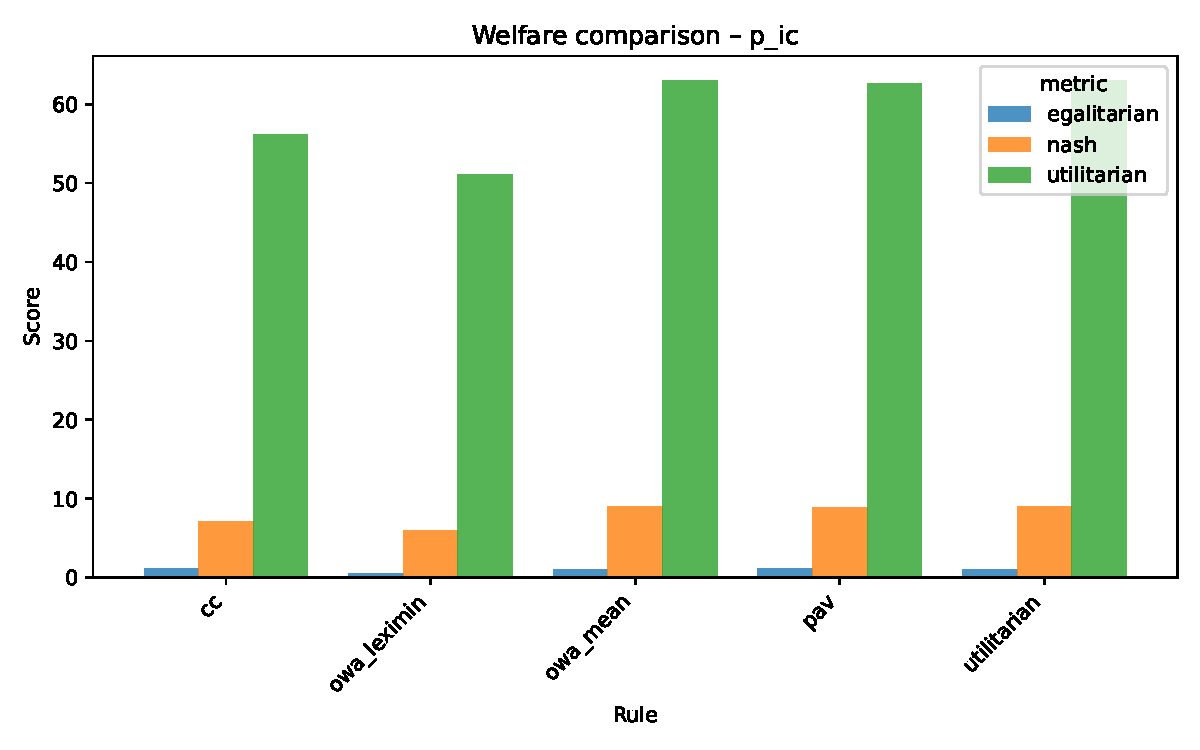
\includegraphics[width=0.7\textwidth]{figures/welfare_comparison_p_ic.pdf}
\caption{Welfare comparison for p-IC culture across voting rules.}
\end{figure}

\begin{figure}[h!]
\centering
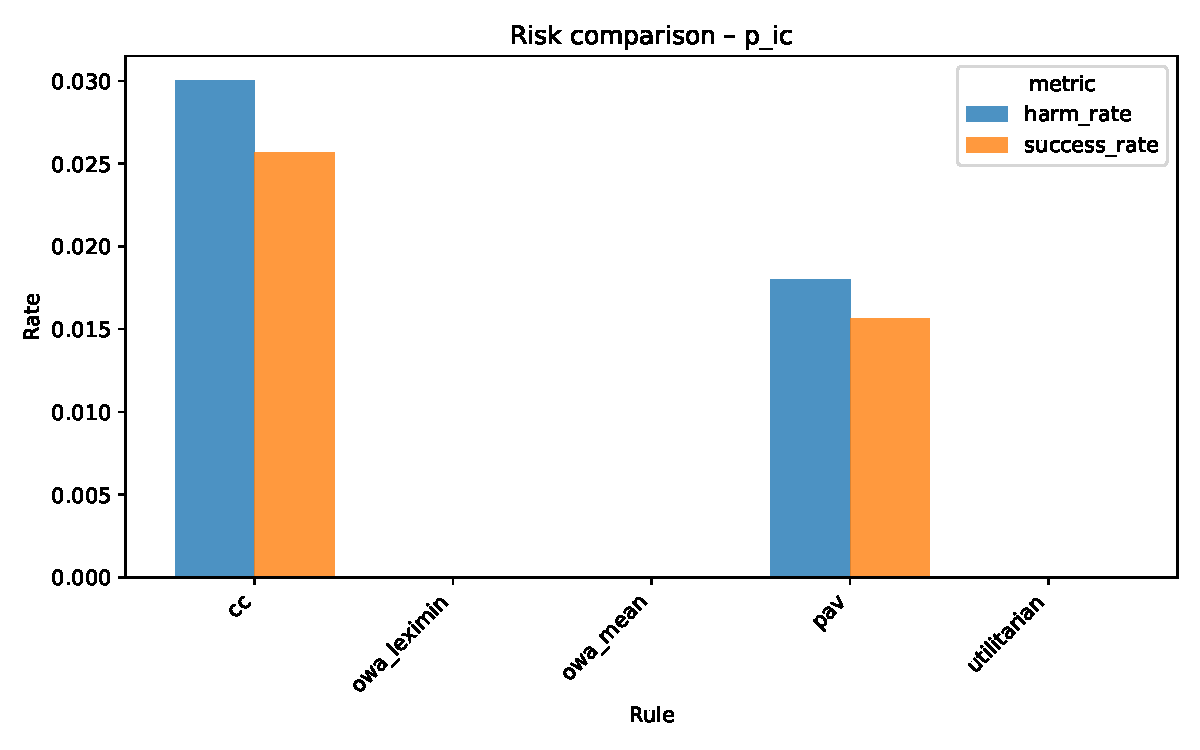
\includegraphics[width=0.7\textwidth]{figures/risk_comparison_p_ic.pdf}
\caption{Manipulation risk under p-IC culture.}
\end{figure}

\subsection{Disjoint Groups}

\begin{figure}[h!]
\centering
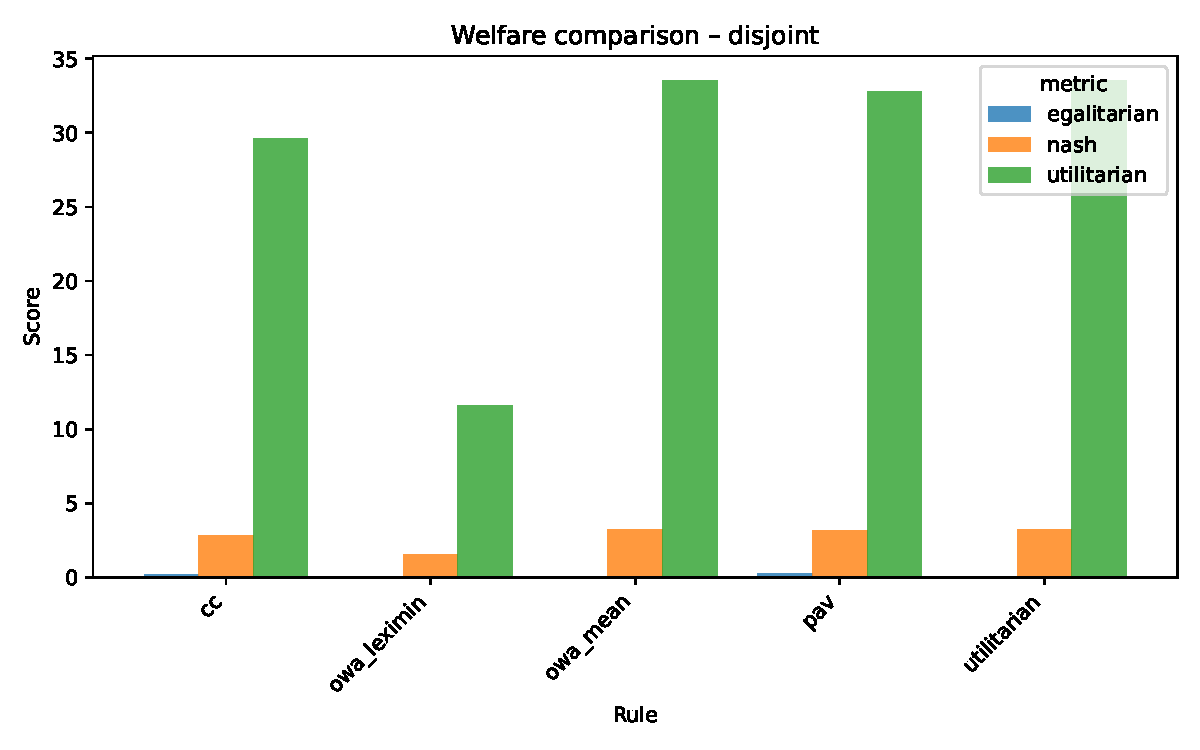
\includegraphics[width=0.7\textwidth]{figures/welfare_comparison_disjoint.pdf}
\caption{Welfare comparison for disjoint-group culture.}
\end{figure}

\begin{figure}[h!]
\centering
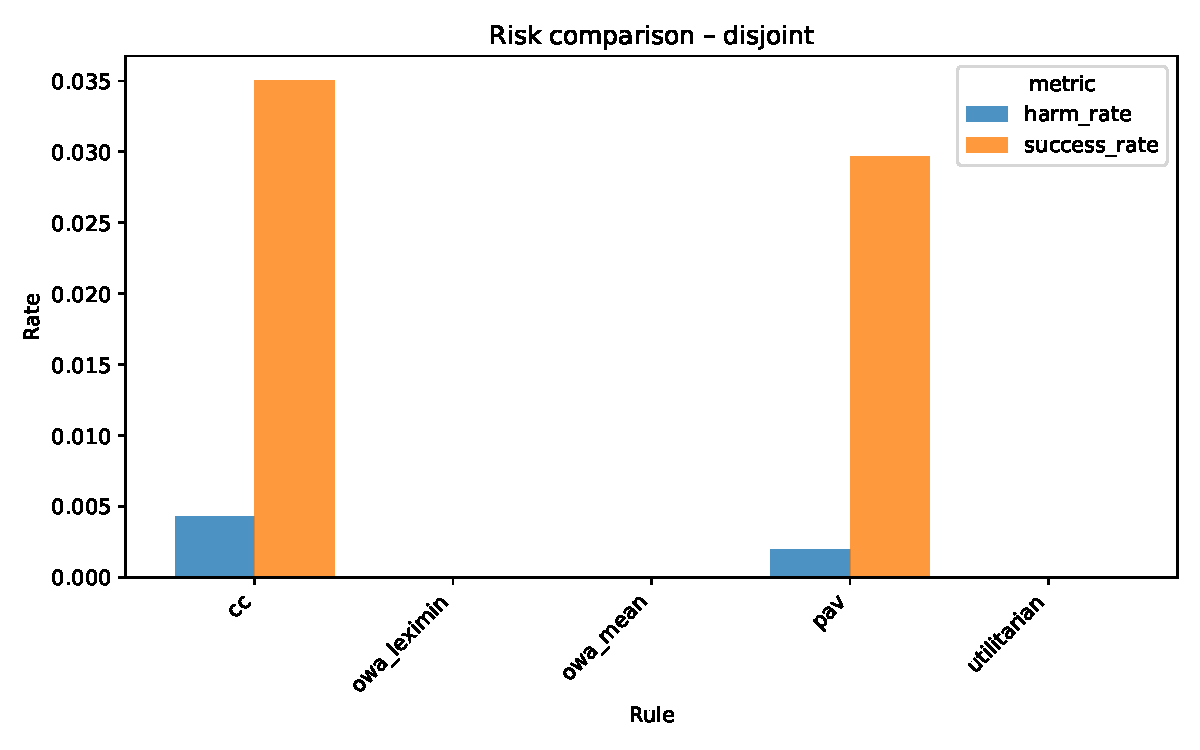
\includegraphics[width=0.7\textwidth]{figures/risk_comparison_disjoint.pdf}
\caption{Manipulation risk under disjoint-group culture.}
\end{figure}

\subsection{Resampling Model}

\begin{figure}[h!]
\centering
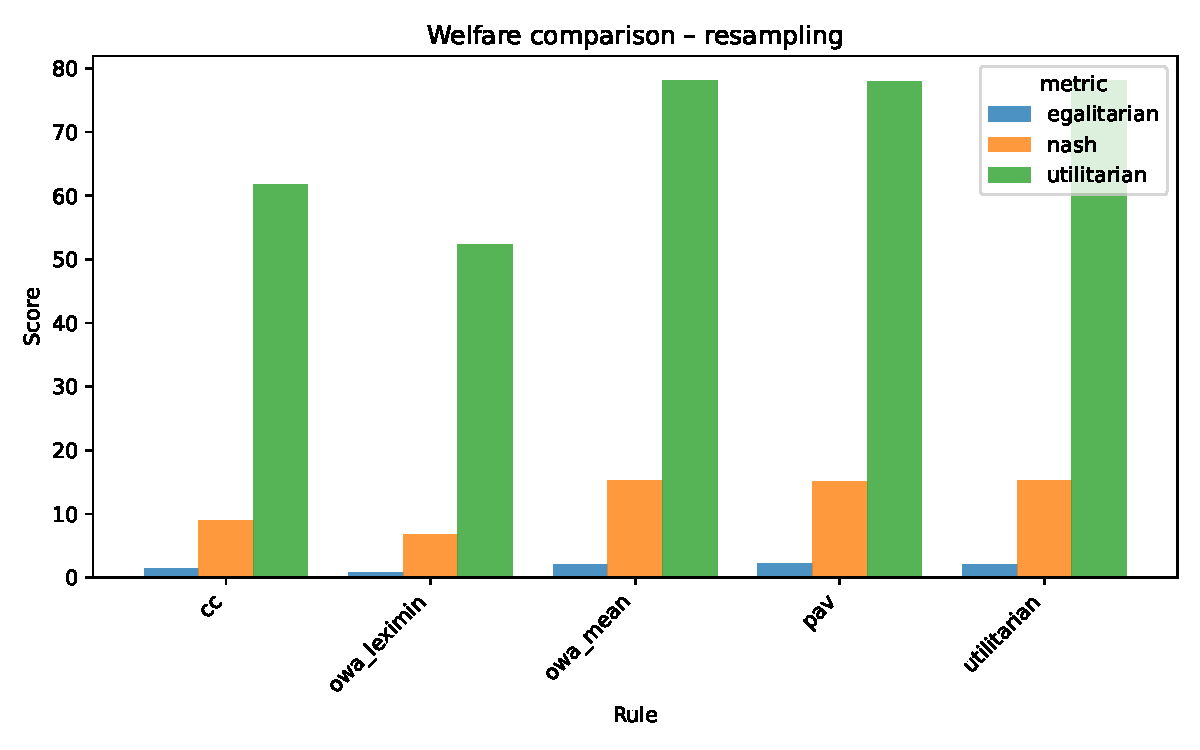
\includegraphics[width=0.7\textwidth]{figures/welfare_comparison_resampling.pdf}
\caption{Welfare comparison for resampling culture.}
\end{figure}

\begin{figure}[h!]
\centering
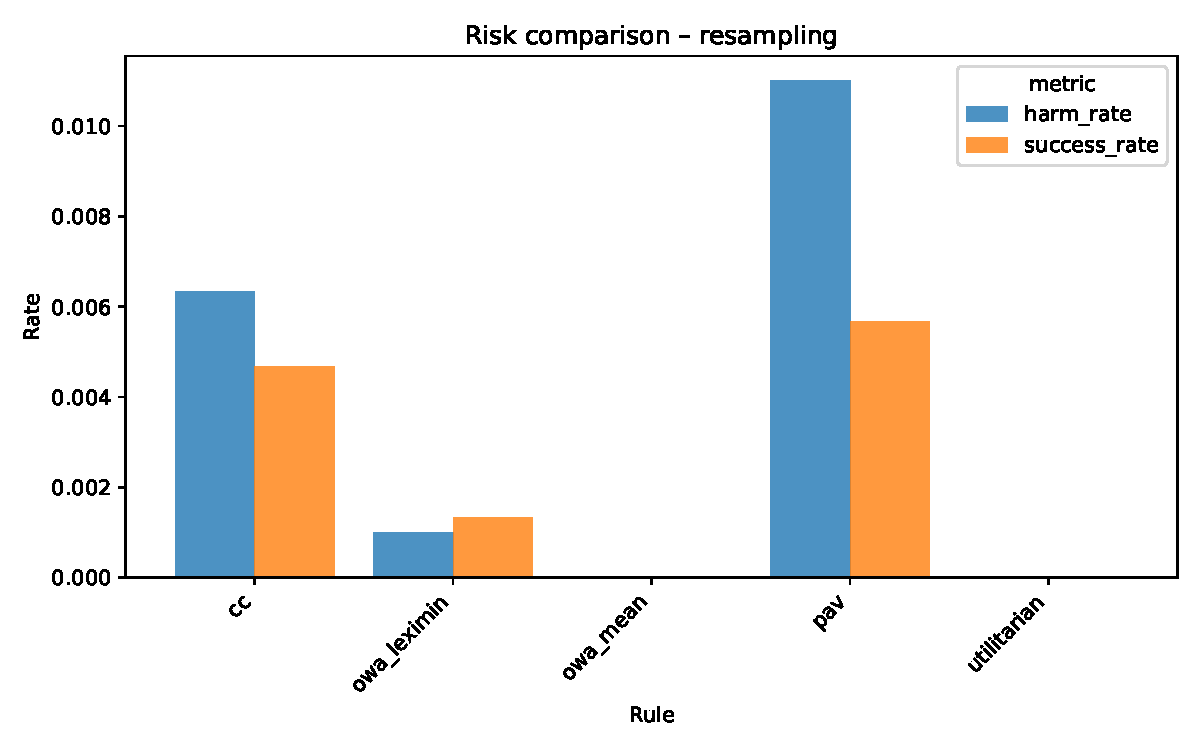
\includegraphics[width=0.7\textwidth]{figures/risk_comparison_resampling.pdf}
\caption{Manipulation risk under resampling culture.}
\end{figure}

\subsection{Hamming Noise}

\begin{figure}[h!]
\centering
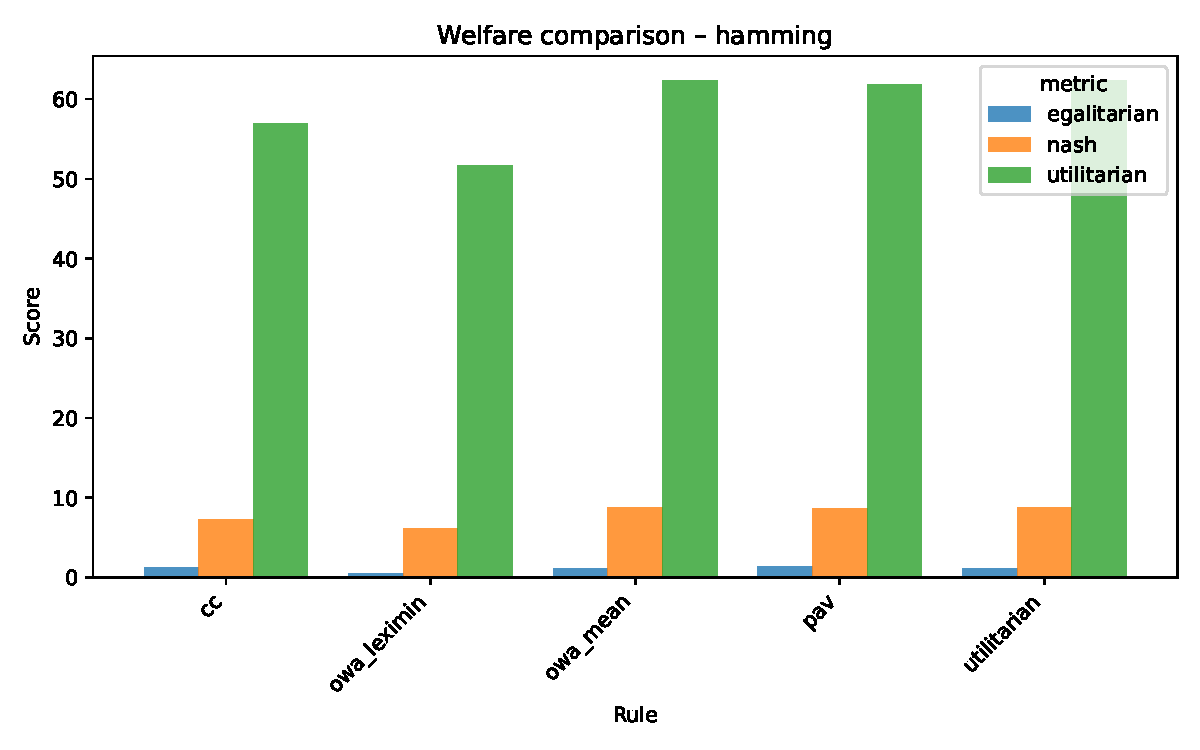
\includegraphics[width=0.7\textwidth]{figures/welfare_comparison_hamming.pdf}
\caption{Welfare comparison for Hamming-noise culture.}
\end{figure}

\begin{figure}[h!]
\centering
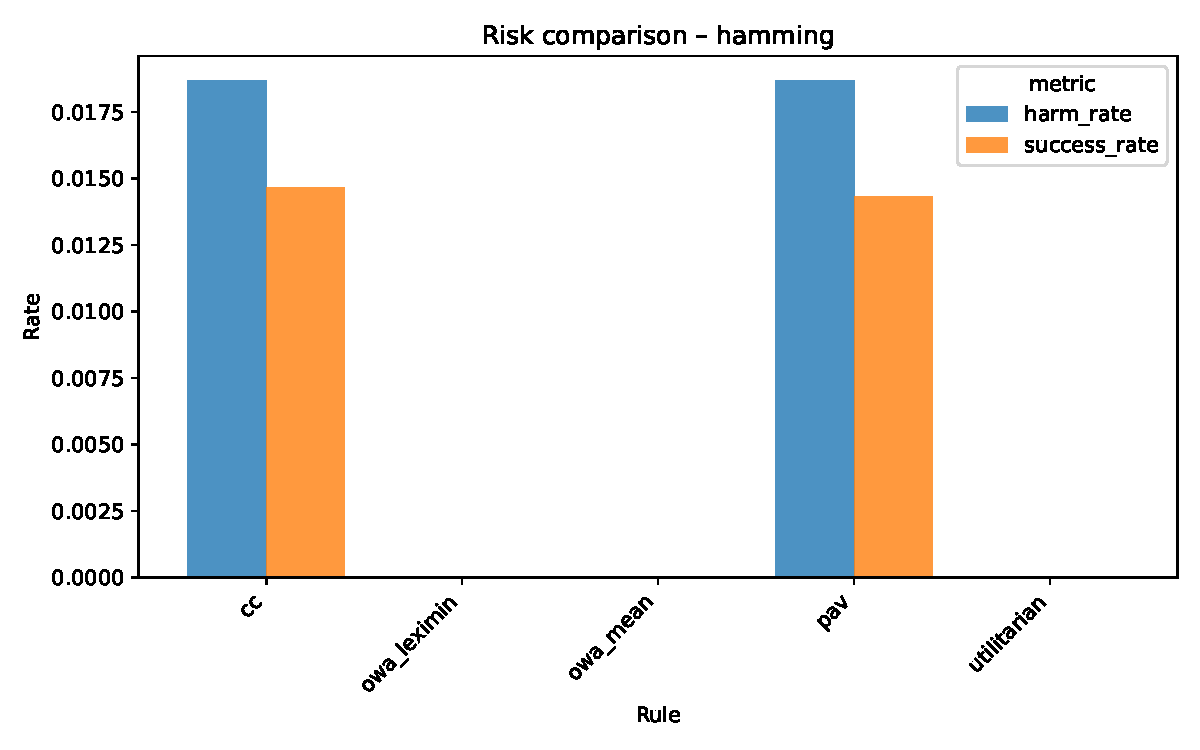
\includegraphics[width=0.7\textwidth]{figures/risk_comparison_hamming.pdf}
\caption{Manipulation risk under Hamming-noise culture.}
\end{figure}

\section{Code Documentation Summary}
\begin{itemize}
  \item \textbf{core/} – Base types, welfare functions, and voting rule interface.
  \item \textbf{statistical\_cultures/} – Preference generators (p-IC, disjoint, resampling, hamming noise).
  \item \textbf{voting\_rules/} – Implementations of utilitarian, PAV, CC, and OWA rules.
  \item \textbf{free\_riding/} – Manipulation detector, welfare/risk analysis tools.
  \item \textbf{experiments/} – Main experiment runner for end-to-end evaluation.
  \item \textbf{tests/} – Unit tests for cultures, rules, and free-riding checks.
\end{itemize}

\bibliographystyle{plain}
\bibliography{references}

\end{document}
% !TEX root = report.tex
